\section{Introduction}

\subsection{Problem Background}

Mass gatherings in stadiums, churches, bus terminals, music festivals, and other venues account for tens of thousands of individuals in a relatively small area. Pedestrian movements in such gatherings are normally orderly and predictable; however, when an unexpected event occurs, a panic outbreak might happen. This leads to rapid increase of the compressive forces between people, which often leads to suffocation in less than a minute in what is called a \textit{crowd crush} rather than stampede \cite{helbing2007dynamics}.

According to Illiyas et al.\ \cite{illiyas2013human}, accidents that occurred in crowds worldwide in 1980--2007 reached 215 major incidents that resulted in over 7{,}000 fatalities. This number grows to 440 incidents and over 13{,}700 fatalities as of 2022. Notable incidents include the 2005 Al-Aimmah Bridge disaster in Baghdad (953 dead), the 2010 Love Parade disaster in Duisburg (21 dead), the 2014 Shanghai New Year's Eve crush (36 dead), and the 2022 Itaewon disaster in Seoul (159 dead). India has seen numerous such tragedies, driven by the massive scale of public gatherings. In July 2024, a stampede at a Hathras religious assembly caused 121 deaths. This was followed by at least 30 fatalities at the Prayagraj Maha Kumbh in January 2025. More recently, in June 2025, 11 people died during the RCB IPL celebration outside Bengaluru's M.\ Chinnaswamy Stadium when a crowd of two lakh supporters gathered, bypassing local security barriers.

From a crowd-dynamics perspective, research has established that densities exceeding 4--5~persons per square metre represent a critical threshold beyond which individuals lose autonomous control of their movement \cite{helbing2007dynamics}. At 6+ persons per square metre, the crowd begins to exhibit fluid-like behaviour, with involuntary pressure waves capable of exerting forces in excess of 4{,}500~N on those pressed against barriers or other bodies. The primary cause of death in nearly all documented incidents is compressive asphyxia---chest compression that prevents respiration---rather than trampling, a distinction that is important for understanding the failure mode that any detection system must target.

What makes these events especially difficult to mitigate is the extremely narrow window of opportunity for intervention. Currently, crowd management relies mostly on human supervision of closed-circuit television (CCTV) cameras. In a typical control room, a single operator might be tasked with watching over 50--100 cameras at once. Thus, the subtle changes in crowd density distribution or sudden local increase of pedestrian speed that happen in the early stages of a disaster might not be noticed in time. When the abnormality becomes apparent to a human operator, the panic outbreak or stampede already happened, and the response team has to deal with the consequences.

This operational gap motivates the development of automated, real-time crowd-anomaly detection systems. A surveillance camera feed is, fundamentally, a time-ordered sequence of pixel intensities. If meaningful motion descriptors can be extracted from that sequence---quantifying how fast people are moving, in which directions, and how much disagreement exists between neighbouring motion vectors---then a classifier can be trained to distinguish normal pedestrian flow from the chaotic, multidirectional scatter that precedes a crush. The challenge, however, lies in achieving this with sufficient accuracy, at processing speeds that permit real-time deployment, and with enough transparency that a human operator can trust and act upon the system's output.

\begin{center}
  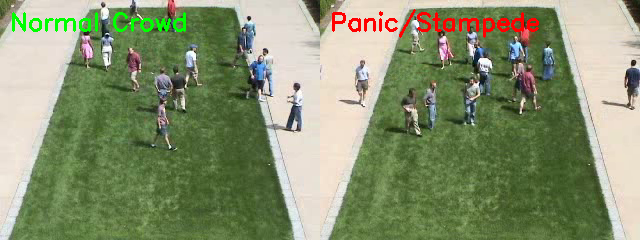
\includegraphics[width=0.85\linewidth]{figures/crowd_example.png}
  \captionof{figure}{Illustrative frames from the UMN Crowd Activity Dataset. \textit{Left:} normal pedestrian flow with consistent, low-speed movement in a shared direction. \textit{Right:} onset of a panic event characterised by high-speed, multidirectional scattering and abrupt changes in crowd density gradients.}
  \label{fig:crowd_example}
\end{center}

\subsection{Research Gap}

Despite these advancements, existing automated crowd-monitoring systems face several key limitations. Handcrafted motion descriptors, such as those relying solely on average flow statistics, lack descriptors for directional coordination or angular agreement. Consequently, they struggle to distinguish between fast, orderly, unidirectional flows and chaotic, multidirectional panic states. In terms of classifier architectures, current recurrent models operate unidirectionally and process sequences with uniform temporal weighting. This prevents the model from leveraging subsequent contextual frames or prioritizing the specific temporal windows where panic behavior begins. Furthermore, explainability is rarely addressed, leaving operators with uninterpretable outputs. Finally, deep learning models often rely on computationally intensive convolutional or Transformer backbones that are unsuitable for real-time edge processing, and they are typically evaluated on single datasets without demonstrating zero-shot generalisation across different environments.

\subsection{Contributions}

The present work addresses these limitations by developing an end-to-end real-time crowd anomaly detection system. The following contributions are made:

\begin{itemize}
  \item A \textbf{nine-feature optical-flow descriptor} is designed by augmenting the baseline three-feature set with six additional statistics (mean, standard deviation, and skewness of flow magnitude; motion coherence; circular variance of flow angles; and motion-density fraction). This expanded descriptor captures speed variability, distributional asymmetry, and directional coordination that baseline descriptors omit.

  \item A recurrent neural architecture is developed that replaces unidirectional LSTMs with a \textbf{Bidirectional LSTM augmented by an additive attention mechanism} (BiLSTM+Attention). This model processes temporal sequences in both forward and reverse directions and assigns learned, non-uniform attention weights to individual time-steps, focusing on the critical early frames of panic rather than averaging over the entire sequence.

  \item A diagnostic \textbf{explainability module} combining permutation feature importance and attention-weight visualization is integrated. This lets operators audit predictions on a per-prediction basis by identifying the most influential flow features and the exact frames that triggered the alert.

  \item Comprehensive empirical validation is performed, including demonstrating \textbf{cross-dataset generalisation} via zero-shot evaluation on the UCSD Ped2 and CUHK Avenue datasets, as well as conducting \textbf{robustness experiments} under synthetic Gaussian noise and motion blur to map the system's operational boundaries.

  \item The pipeline is demonstrated to be highly suitable for real-time edge hardware, achieving an execution speed of \textbf{54.5 frames per second} on a consumer-grade laptop GPU (NVIDIA RTX 4050) with a footprint of only 554{,}817 parameters (over 40$\times$ smaller than ResNet-50).
\end{itemize}

The rest of this paper is structured as follows. Section~2 contains the literature review. Section~3 details the methodology, covering the features, classifier architecture, and explainability modules. Section~4 outlines the experimental setup, while Section~5 presents the empirical results. Finally, Section~6 provides a discussion of the findings, and Section~7 outlines conclusions and future research paths.
